\section{Performance Evaluation}
\label{sec:performance}
To evaluate \textsc{Synopsis}, we used a real-world dataset to populate the distributed sketch. This includes dynamic scaling and an analysis of node stability as scaling operations take place, as well as query evaluation latencies for each query type.

\subsection{Dynamic Scaling}
\begin{figure}
    \centerline{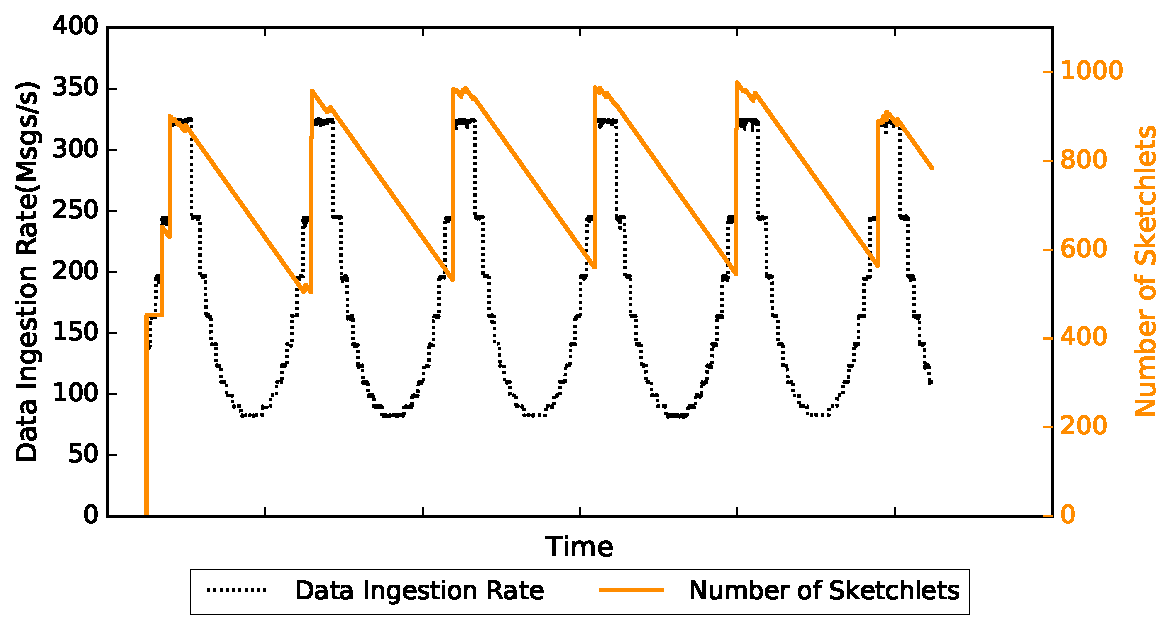
\includegraphics[width=3.5in]{figures/dyn-scaling.pdf}}
    \caption{The variation of number of sketchlets with the data ingestion rate.}
    \label{fig:dyn-scaling}
\end{figure}
We evaluated how \textsc{Synopsis} dynamically scales when the data ingestion rate is varied.
The data ingestion rate was varied over time such that the peak data ingestion rate is less than the highest possible throughput that will create a backlog at \textsc{Synopsis} nodes.
We used the number of sketchlets created in the system to quantify the scaling activities.
If the system scales out, more sketchlets will be created in child nodes after the targeted load migration.
We started with a single \textsc{Synopsis} node and allowed the system to dynamically scale.
As can be observed in Figure~\ref{fig:dyn-scaling}, the number of sketchlets varies with the ingestion rate.
Since we allow aggressive scale out, it shows a rapid scale out activity during high data ingestion rates whereas scaling in takes place gradually with one sub region (hence one sketch) at a time.


\subsection{Stability at Individual Nodes}
The objective of this benchmark was to demonstrate how scaling out operations manage to maintain stability at each node under varying workload conditions.
The same setup as in previous micro benchmark was used, but the evaluation metrics captured are corresponding to an individual node instead of the entire system.
For this experiment, we have enabled only a single threshold-based rule (either backlog growth based or memory usage based) at a time to demonstrate its effectiveness.



